	Any state-transition model contains a set of Variables. Each variable contains a reference to a question type (e.g. Single, Multiple, Open or grid) and its operand type, i.e. the data gathered for that question. As each question has a concrete implementation of Variable (e.g. VariableSingle, VariableMultiple, VariableOpen or VariableGrid), we have decided to implement the factory pattern. This creational pattern permits abstracting the concrete instantiation of the variables through the Variable interface but and reduces the need to modify code if a new question type is added to the \gls{cawi} system.

	The Figure \ref{fig:design:factoryPattern} represents the relations and classes needed to implement this pattern. The client asks for the creation of a Variable by passing a concrete question to the VariableFactory (e.g. a Multiple question). This pattern decides what is the adequate Variable for that question (e.g. VariableMultiple) and creates an object that contains the operand associated to that Variable (e.g. OperandMap that reflects a set of keys and boolean values to represent the responses codes for a question and determining whether that code has been selected or not). This pattern is currently used by the parser package (explained in Section \ref{sec:design:businessLayer}) and abstracts the creation of variables for each question defined at any \gls{xml} instance.

	\begin{figure}[H]
	\centering
	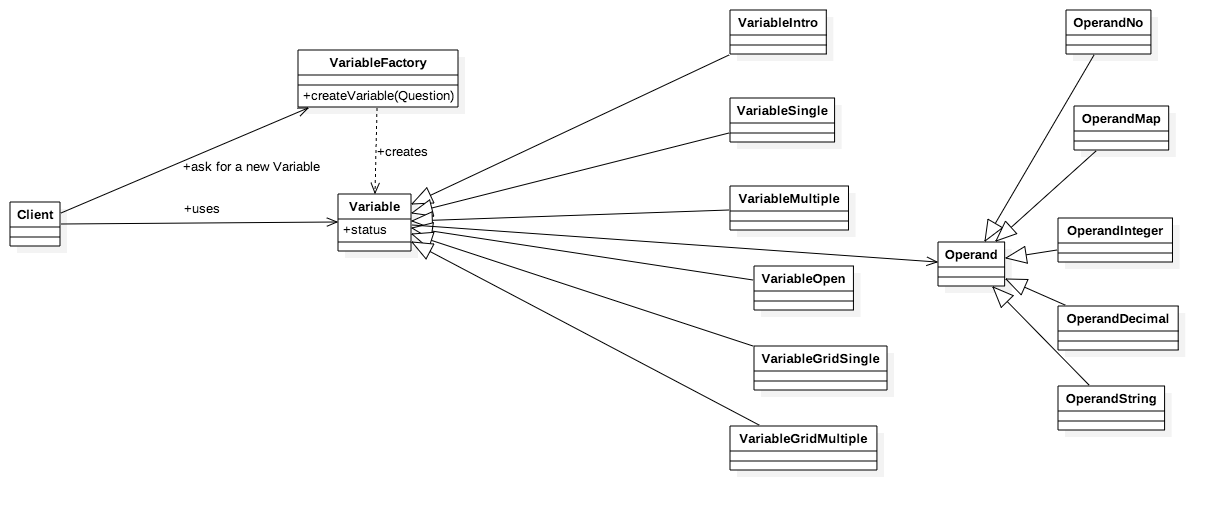
\includegraphics[max size={\textwidth}{\textheight}]{design/img/variableFactory.png}
	\caption{Factory Design Pattern for creating Variables}
	\label{fig:design:factoryPattern}
	\end{figure}

	

